% Options for packages loaded elsewhere
\PassOptionsToPackage{unicode}{hyperref}
\PassOptionsToPackage{hyphens}{url}
\documentclass[
]{article}
\usepackage{xcolor}
\usepackage{amsmath,amssymb}
\setcounter{secnumdepth}{-\maxdimen} % remove section numbering
\usepackage{iftex}
\ifPDFTeX
  \usepackage[T1]{fontenc}
  \usepackage[utf8]{inputenc}
  \usepackage{textcomp} % provide euro and other symbols
\else % if luatex or xetex
  \usepackage{unicode-math} % this also loads fontspec
  \defaultfontfeatures{Scale=MatchLowercase}
  \defaultfontfeatures[\rmfamily]{Ligatures=TeX,Scale=1}
\fi
\usepackage{lmodern}
\ifPDFTeX\else
  % xetex/luatex font selection
\fi
% Use upquote if available, for straight quotes in verbatim environments
\IfFileExists{upquote.sty}{\usepackage{upquote}}{}
\IfFileExists{microtype.sty}{% use microtype if available
  \usepackage[]{microtype}
  \UseMicrotypeSet[protrusion]{basicmath} % disable protrusion for tt fonts
}{}
\makeatletter
\@ifundefined{KOMAClassName}{% if non-KOMA class
  \IfFileExists{parskip.sty}{%
    \usepackage{parskip}
  }{% else
    \setlength{\parindent}{0pt}
    \setlength{\parskip}{6pt plus 2pt minus 1pt}}
}{% if KOMA class
  \KOMAoptions{parskip=half}}
\makeatother
\usepackage{longtable,booktabs,array}
\usepackage{calc} % for calculating minipage widths
% Correct order of tables after \paragraph or \subparagraph
\usepackage{etoolbox}
\makeatletter
\patchcmd\longtable{\par}{\if@noskipsec\mbox{}\fi\par}{}{}
\makeatother
% Allow footnotes in longtable head/foot
\IfFileExists{footnotehyper.sty}{\usepackage{footnotehyper}}{\usepackage{footnote}}
\makesavenoteenv{longtable}
\usepackage{graphicx}
\makeatletter
\newsavebox\pandoc@box
\newcommand*\pandocbounded[1]{% scales image to fit in text height/width
  \sbox\pandoc@box{#1}%
  \Gscale@div\@tempa{\textheight}{\dimexpr\ht\pandoc@box+\dp\pandoc@box\relax}%
  \Gscale@div\@tempb{\linewidth}{\wd\pandoc@box}%
  \ifdim\@tempb\p@<\@tempa\p@\let\@tempa\@tempb\fi% select the smaller of both
  \ifdim\@tempa\p@<\p@\scalebox{\@tempa}{\usebox\pandoc@box}%
  \else\usebox{\pandoc@box}%
  \fi%
}
% Set default figure placement to htbp
\def\fps@figure{htbp}
\makeatother
\ifLuaTeX
  \usepackage{luacolor}
  \usepackage[soul]{lua-ul}
\else
  \usepackage{soul}
\fi
\setlength{\emergencystretch}{3em} % prevent overfull lines
\providecommand{\tightlist}{%
  \setlength{\itemsep}{0pt}\setlength{\parskip}{0pt}}
% ---- Custom preamble additions injected by pandoc (-H) ----
% Map the few non-ASCII symbols that appear in body text so the document
% compiles under pdfLaTeX (default Overleaf engine) as well as XeLaTeX/LuaLaTeX.
\usepackage{newunicodechar}
\newunicodechar{±}{\ensuremath{\pm}}
\newunicodechar{−}{\ensuremath{-}}
\newunicodechar{→}{\ensuremath{\rightarrow}}
\newunicodechar{×}{\ensuremath{\times}}
\newunicodechar{∈}{\ensuremath{\in}}
\newunicodechar{ε}{\ensuremath{\varepsilon}}
\newunicodechar{ē}{\ensuremath{\bar{e}}}
\newunicodechar{；}{;}
\newunicodechar{？}{?}

% Figures live in ./figures
\graphicspath{{figures/}}
\usepackage{bookmark}
\IfFileExists{xurl.sty}{\usepackage{xurl}}{} % add URL line breaks if available
\urlstyle{same}
\hypersetup{
  hidelinks,
  pdfcreator={LaTeX via pandoc}}

\author{}
\date{}

\begin{document}

\section{Exploring Equilibrium Efforts in Rank-Order Tournaments via
Policy-Gradient
Self-Play}\label{exploring-equilibrium-efforts-in-rank-order-tournaments-via-policy-gradient-self-play}

\textbf{Abstract}

Rank-order tournaments are a canonical model of strategic effort under
uncertainty, but equilibrium analysis becomes increasingly difficult
once tournament environments move beyond the analytically tractable
one-stage setting. This paper explores whether a learning-based solver
can recover tournament equilibrium effort from self-play interaction and
thereby provide a computational foundation for settings in which
closed-form analysis is unavailable.

We propose Tournament Equilibrium Learning via PPO (TEL-PPO), a
self-play policy-gradient framework that models the one-stage tournament
as a one-shot stochastic game with bounded continuous actions. TEL-PPO
uses Beta-parameterized effort policies and augments self-play
optimization with explicit equilibrium-quality checks based on stability
diagnostics and exploitability estimation.

We evaluate the method in the canonical Lazear-Rosen one-stage
tournament, where analytical equilibrium effort is available as ground
truth, and compare it with a Monte Carlo finite-difference gradient
baseline in the tractable setting. Across symmetric, multi-player, and
heterogeneous tournament variants, TEL-PPO recovers the correct
equilibrium structure in stable cases and remains close to the
theoretical benchmark when the proposed equilibrium-quality diagnostics
are satisfied. At the same time, the controlled one-stage setting
provides a useful benchmark for distinguishing between training
stabilization, low exploitability, and accurate recovery of the
analytical equilibrium.

These findings establish the one-stage tournament as a useful validation
benchmark for learning-based equilibrium computation and show that
explicit equilibrium verification is essential before extending
self-play methods to analytically intractable multi-stage or
higher-dimensional tournament environments.

\textbf{Keywords:} Rank-order tournaments, equilibrium computation,
self-play, reinforcement learning, PPO

\begin{enumerate}
\def\labelenumi{\arabic{enumi}.}
\item
  \textbf{Introduction \& Motivation}
\end{enumerate}

Rank-order tournaments are a canonical model of strategic effort under
uncertainty, in which agents exert costly effort to improve relative
performance and rewards are assigned by rank rather than absolute
output. Since the seminal work of Lazear and Rosen {[}1{]}, tournament
models have provided a standard framework for analyzing incentive design
and equilibrium effort in rank-based competitive environments.

Despite their analytical appeal, tournament models become difficult to
solve once the environment moves beyond the canonical one-stage setting.
Closed-form equilibrium characterization is typically available only
under restrictive assumptions, such as simple noise structures,
symmetric agents, or static interaction. When tournament environments
incorporate multiple stages, heterogeneous participants, asymmetric cost
structures, or more complex strategic dependencies, analytical
equilibrium derivation becomes increasingly difficult and is often
unavailable. As a result, many tournament environments of practical
interest lack a tractable computational procedure for equilibrium
characterization.

This paper examines whether a learning-based solver can recover
tournament equilibrium effort in the analytically tractable one-stage
setting, thereby providing a credible starting point for extension to
more complex tournament environments. We focus on this question because
the one-stage Lazear-Rosen tournament admits an analytical equilibrium
benchmark {[}1{]}, making it possible to validate whether a self-play
learning method converges to the correct fixed point before applying it
to settings where closed-form solutions are unavailable.

Recent advances in deep reinforcement learning, particularly in
self-play methods, have provided a computational approach for solving
complex strategic environments through repeated interaction rather than
explicit analytical derivation. In stochastic competitive settings with
continuous actions, learning agents can adapt to noisy outcomes and
strategic opponents while improving their policies over time. This makes
reinforcement learning a natural candidate for tournament environments,
where agents choose effort strategically, realized outcomes are noisy,
and performance depends on relative rank rather than absolute output.
The challenge, however, is not merely optimization under uncertainty,
but whether self-play can recover equilibrium effort in a rank-order
stochastic contest. Among policy-gradient methods, Proximal Policy
Optimization (PPO) offers a stable and scalable framework for
continuous-action learning {[}2{]}.

Motivated by this perspective, we propose the Tournament Equilibrium
Learning Framework based on Proximal Policy Optimization (TEL-PPO), a
self-play policy-gradient approach for equilibrium effort computation in
rank-order tournaments. TEL-PPO models the one-stage tournament as a
one-step stochastic game with continuous bounded effort actions and
combines Beta-parameterized policies with explicit equilibrium
verification based on stability diagnostics and exploitability
estimation.

The purpose of the one-stage setting in this paper is not to revisit a
solved model, but to use it as a controlled validation benchmark for a
learning-based equilibrium solver. By comparing learned effort profiles
with a benchmark of known equilibrium structure, we can test whether
self-play recovers the correct fixed point before extending the approach
to tournament environments in which analytical characterization may be
unavailable.

This paper makes three contributions. First, we cast equilibrium-effort
computation in noisy rank-order tournaments as a self-play learning
problem with bounded continuous actions. Second, we develop TEL-PPO, a
PPO-based framework that combines self-play learning with explicit
equilibrium-quality diagnostics, including stability screening and
exploitability checks. Third, using the analytically solvable one-stage
tournament as a benchmark, we show that TEL-PPO recovers the correct
equilibrium structure in stable regimes and that explicit verification
is necessary because optimization stability, low exploitability, and
benchmark accuracy do not always coincide.

The remainder of this paper is organized as follows: Section 2 reviews
related work. Section 3 introduces the tournament model and the
analytical benchmark. Section 4 presents TEL-PPO and the gradient-based
baseline. Section 5 reports the experimental results and diagnostic
analyses. Section 6 concludes and discusses future directions.

\begin{enumerate}
\def\labelenumi{\arabic{enumi}.}
\setcounter{enumi}{1}
\item
  \textbf{Related work}
\end{enumerate}

\subsection{\texorpdfstring{\textbf{2.1 Background on Tournaments and
Analytical Contest
Models}}{2.1 Background on Tournaments and Analytical Contest Models}}\label{background-on-tournaments-and-analytical-contest-models}

Contests provide a fundamental framework in economics and management for
studying competitive environments in which agents exert costly effort to
compete for predetermined rewards. Canonical contest models include the
Tullock contest {[}3{]}, the Lazear-Rosen rank-order tournament {[}1{]},
and the all-pay auction {[}4{]}. These frameworks differ in how effort
is translated into competitive outcomes, but together they form the
foundation of the modern contest literature.

In Tullock contests, the probability of winning is proportional to an
individual's effort relative to aggregate effort, making the model well
suited to applications such as rent-seeking, R\&D competition, and
political campaigns {[}3{]}. In all-pay auctions, all contestants pay
their bid regardless of the outcome, and the framework has been widely
used to study lobbying, conflict, and crowdsourcing competition {[}4{]}.
By contrast, the Lazear-Rosen tournament assigns rewards according to
relative rank rather than absolute output, with realized performance
subject to stochastic shocks {[}1{]}. This formulation has been
especially influential in labor economics and organizational design,
where it provides a benchmark model for studying promotion incentives,
wage dispersion, and strategic effort under relative-performance
evaluation.

Among these frameworks, the rank-order tournament is particularly
relevant for the present study because it combines strategic effort
choice with stochastic performance comparison. In the canonical
one-stage setting, the Lazear-Rosen model admits an analytically
tractable benchmark for equilibrium effort {[}1{]}. However,
tractability deteriorates quickly as contests become more elaborate, for
example through multistage structure or richer heterogeneity, noise,
cost, or information assumptions. Subsequent theoretical work has
extended canonical contest formulations in several directions. For
example, {[}5{]} derives closed-form optimal bias of the contest rule in
asymmetric \(n\)-player contests with heterogeneous contestants, while
{[}6{]} shows that general two-player contests with heterogeneous skill
distribution can admit a symmetric equal-effort equilibrium under broad
assumption on production technology and skill distributions. These
studies illustrate both the reach and the limits of analytical modeling:
it can yield sharp equilibrium characterizations in structured
environments, but it does not by itself furnish a general computational
procedure for equilibrium recovery in more complex tournament settings.

\subsection{\texorpdfstring{\textbf{2.2 Empirical and Experimental
Research on
Contests}}{2.2 Empirical and Experimental Research on Contests}}\label{empirical-and-experimental-research-on-contests}

Empirical and experimental research complements analytical contest
theory by examining how contestants respond to alternative tournament
designs in practice. Experimental studies have explored how effort
varies with prize allocation, tournament size, and the proportion of
winners {[}7{]}. In particular, Harbring and Irlenbusch {[}8{]} and
Knauer et al. {[}9{]} show that increasing the share of winners can
raise average effort, while Harbring and Irlenbusch {[}8{]} also find
that very small tournaments, especially two-player tournaments, may be
more prone to collusive behavior. Field studies further show that
observed performance depends not only on incentive structure but also on
characteristics of the competitive environment. In professional golf,
the presence of a superstar can discourage rivals and reduce performance
{[}10{]}. In auto racing, tournament prize spreads affect both
performance and safety, although prize distribution itself appears less
important once the size of the spread is controlled for {[}11{]}.
Experimental evidence also shows that proportional-prize contests can
induce effort above Nash benchmarks, although they generally produce
lower effort and more equitable payoffs than winner-take-all contests
{[}12{]}.

For our purposes, the main limitation of this literature is
methodological. Empirical and experimental studies provide valuable
evidence on behavior under alternative contest designs, but they do not
by themselves provide a general computational framework for recovering
equilibrium behavior in strategically rich tournament environments.

\textbf{2.3 Reinforcement Learning for Equilibrium Approximation in
Strategic Environments}

The limitations of analytical approaches motivate the use of
computational methods for equilibrium approximation in strategic
environments where closed-form solutions are unavailable. In particular,
multi-agent reinforcement learning (MARL) provides a flexible framework
in which strategic behavior can emerge through repeated interaction,
self-play, and adaptation to other agents. Surveys on multi-agent deep
reinforcement learning document a broad range of techniques for
competitive and cooperative environments and highlight their usefulness
in high-dimensional and stochastic games {[}13{]}.

\emph{\textbf{RL in Contest-Like Environments.}} Reinforcement learning
has already been applied to several competitive environments that share
structural similarities with contests. For example, {[}14{]} propose the
BRAT and Meta\_Nash DQN agents to approximate Nash equilibria in
two-player simultaneous-action games using joint-action deep Q-learning.
More broadly, {[}15{]} studies the computational performance of deep
reinforcement learning for finding Nash equilibria, while {[}16{]}
applies multi-agent deep reinforcement learning to approximate
equilibrium behavior in day-ahead electricity market bidding games.
Other work combines fictitious play with deep reinforcement learning to
approximate equilibria in imperfect-information games without prior
domain knowledge {[}17{]}. These studies show that learning-based
methods can recover strategic behavior in settings where equilibrium
computation is analytically difficult.

Multi-agent learning has also been applied to contest-like mechanisms
more directly. For example, {[}18{]} develops a deep-learning and
multi-agent simulation framework for designing all-pay auctions. These
applications demonstrate that reinforcement learning can be used to
study structured competitive environments, although many of them involve
payoff structures that are smoother or more directly tied to actions
than in the rank-order tournament considered here, where stochastic
ranking plays a more central role.

\emph{\textbf{RL for Equilibrium Approximation in Broader Strategic
Settings.}} Beyond contest settings, deep reinforcement learning has
been used to approximate game-theoretic equilibria in a broader range of
strategic environments. Examples include reinforcement-learning methods
for obtaining Nash equilibria in multiplayer matrix games {[}19{]},
DRL-based algorithms for computing Stackelberg-Nash equilibria in
general-sum Markov games {[}20{]}, and broader recent overviews
connecting game-theoretic equilibrium concepts with multi-agent
reinforcement learning {[}21{]}. This literature establishes
reinforcement learning as a general computational framework for
approximating equilibria in games with nonlinear, discontinuous, or
analytically intractable payoff structures.

Despite this progress, noisy rank-order tournaments remain underexplored
from a reinforcement-learning perspective. Relative to Tullock contests
or auction-based settings, the Lazear-Rosen tournament presents a more
challenging structure: rewards are rank-based, performance is
stochastic, and effort affects outcomes through noisy comparisons rather
than through a smooth deterministic contest-success function. This makes
equilibrium computation sensitive to the distribution of performance
shocks and complicates both analytical characterization and numerical
approximation.

This paper addresses that gap by formulating equilibrium-effort
computation in rank-order tournaments as a self-play learning problem
with bounded continuous actions in a one-step stochastic game. We
propose TEL-PPO, a PPO-based framework for learning tournament effort
policies under noisy rank-order incentives. The role of the analytically
solvable one-stage tournament is methodological: because equilibrium
effort is known in closed form in this setting {[}1{]}, it provides a
controlled benchmark for validating whether a learning-based solver
recovers the correct equilibrium structure before being extended to more
complex environments. In this sense, our contribution is not to replace
analytical theory in the tractable case, but to establish a validated
computational foundation for future work on tournament settings in which
closed-form equilibrium analysis is unavailable.

\begin{enumerate}
\def\labelenumi{\arabic{enumi}.}
\setcounter{enumi}{2}
\item
  \textbf{Tournament model and Analytical Benchmark}
\end{enumerate}

We begin with the canonical one-stage rank-order tournament introduced
by Lazear and Rosen {[}1{]}, which serves as the analytical benchmark
throughout this paper. In this environment, two risk-neutral contestants
choose costly effort levels and compete for rank-based rewards
determined by relative performance rather than absolute output.

In the classical one-stage setting, contestants are assumed to be
identical in ability and fully rational. Each player
\(i \in \{ 1,2\}\)chooses an effort level \(e_{i} \geq 0\) to maximize
expected utility. Realized performance depends on both effort and luck,
and is given by

\(y_{i} = e_{i}\) + \(\varepsilon_{i}\), with
\(\varepsilon_{i}\sim U\lbrack - q,\ q\rbrack\) (1)

where \(e_{i}\) denotes the effort chosen by contestant \(i\), and
\(\varepsilon_{i}\) is an additive noise term capturing measurement
error, unobserved fluctuations, or environmental uncertainty. The
uniform-noise specification is standard in the benchmark tournament
model and yields a simple closed-form expression for equilibrium effort.
The presence of noise implies that greater effort increases, but does
not guarantee, the probability of outperforming the opponent.

Rewards are assigned according to rank. Let \(w_{H}\) denote the prize
for the winner and \(w_{L}\) the prize for the loser, with
\(w_{H} > w_{L}\). Effort is costly, and we assume the standard
quadratic cost function

\(c\left( e_{i} \right) = ke_{i}^{2}\) (2)

where \(k > 0\) is the marginal cost parameter. The one-stage payoff of
player \(i\) is therefore

\(u_{i}\) = \(w_{i} - c\left( e_{i} \right),\ \) (3)

where \(w_{i} \in \{ w_{H},\ w_{L}\}\) depends on the contest outcome.
In expectation, the payoff can be written as

\(Eu_{i}\left( e_{i},\ e_{- i} \right) = \ w_{L} + \ p\left( e_{i},\ e_{- i} \right)\left\lbrack w_{H} - \ w_{L} \right\rbrack - \ ke_{i}^{2}\ \ \ \)
(4)

where \(p\left( e_{i},\ e_{- i} \right)\) is the probability that player
\(i\) wins against player \(- i\).

Under the standard symmetric one-stage formulation, solving the
first-order condition yields the closed-form Nash equilibrium effort
{[}22{]}:

\(e^{*} = \ \frac{w_{H} - \ w_{L}}{4qk}\) (5)

In this paper, the closed-form solution is used only as an analytical
benchmark for validation. It does not enter training, policy updating,
or equilibrium computation. The role of the one-stage tournament is
therefore methodological: it provides a controlled benchmark with known
equilibrium structure for testing whether a learning-based solver can
recover the correct solution before being extended to analytically
intractable settings.

\begin{enumerate}
\def\labelenumi{\arabic{enumi}.}
\setcounter{enumi}{3}
\item
  \textbf{Methodology}
\end{enumerate}

\textbf{4.1 Overview}

We propose Tournament Equilibrium Learning with Proximal Policy
Optimization (TEL-PPO), a self-play reinforcement-learning framework for
computing approximate equilibrium effort profiles in rank-order
tournaments. We evaluate TEL-PPO in the analytically tractable one-stage
setting, where it can be compared against two benchmarks: the
closed-form equilibrium effort from the classical Lazear--Rosen
tournament model {[}22{]}, and a simulation-based numerical baseline
obtained via Monte Carlo finite-difference gradient ascent.

Our objective is to determine whether a learning-based method can
recover the equilibrium structure of tournament competition across a
range of settings, including symmetric, heterogeneous, and multi-player
variants. To this end, we assess TEL-PPO along two dimensions: (1)
whether self-play converges to a stable policy profile, and (2) whether
the resulting effort levels agree with theoretical or numerical
equilibrium benchmarks.

A central feature of our framework is the strict separation between
training information and evaluation information. During training,
TEL-PPO observes only sampled contest outcomes and realized rewards. It
does not use closed-form winning probabilities, expected-payoff
formulas, or equilibrium characterizations. These analytical objects are
introduced only after training for evaluation. This design ensures that
any equilibrium recovery arises from interaction-driven learning rather
than from analytical supervision, and it enables a clean distinction
between stable optimization dynamics and genuine equilibrium quality.

\textbf{4.2 TEL-PPO Framework}

TEL-PPO models the tournament as a one-step stochastic game with
continuous bounded effort actions. In each episode, players choose
effort levels, receive noisy performance realizations, obtain rank-based
rewards, and update their policies from observed outcomes. This
formulation is well aligned with rank-order tournaments environments,
where payoffs depend on stochastic relative performance rather than on
smooth deterministic mappings from effort to utility.

We adopt Proximal Policy Optimization (PPO) {[}2{]} as the underlying
policy-gradient method. PPO provides a robust actor-critic framework for
continuous-action learning, and its clipped surrogate objective helps
stabilize policy updates during self-play. This property is especially
important in in competitive stochastic environments, where unconstrained
updates can amplify non-stationarity and destabilize learning.

As shown in Figure 1, the TEL-PPO pipeline consists of three components:
state construction, the self-play environment, and convergence
verification. Given tournament primitives such as prize levels and noise
parameters, TEL-PPO trains two agents through repeated self-play and
periodically evaluate the current policy profile using stability and
exploitability diagnostics. Equilibrium behavior is therefore not
specified a priori but is instead expected to emerge from self-play and
then pass a separate verification procedure. The following subsections
describe these components in detail.

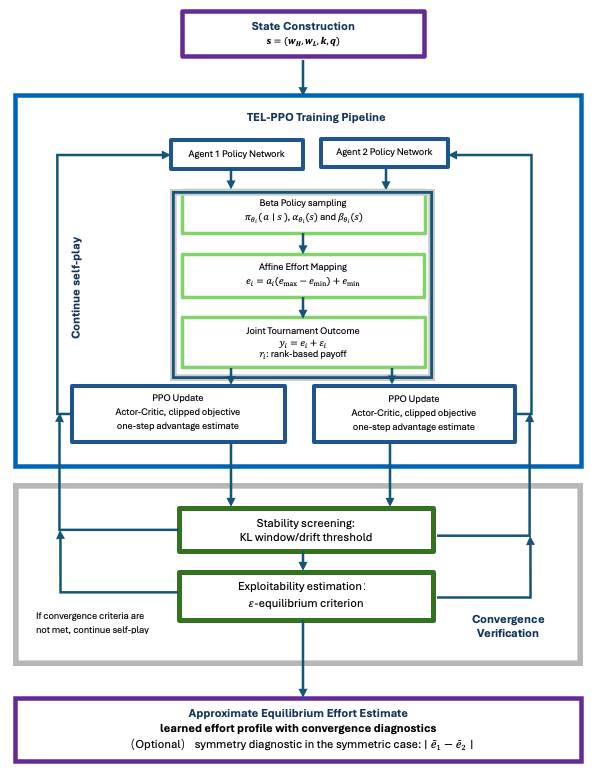
\includegraphics[width=0.55\linewidth]{figures/fig1_framework.png}

\textbf{Figure 1: TEL-PPO framework (Illustration for the two-agent
one-stage setting).}

TEL-PPO models the one-stage rank-order tournament as a one-step
stochastic game with continuous bounded effort actions. Two agents learn
Beta-parameterized effort policies through repeated self-play, receive
rank-based rewards from noisy performance comparisons, and update their
policies using PPO. Training is periodically evaluated through
convergence verification, including stability screening and
exploitability estimation, so that equilibrium recovery is assessed not
only by optimization behavior but also by approximate game-theoretic
consistency. Symmetry is evaluated only after convergence has been
verified.

\textbf{I. State Construction}

In the one-stage tournament, the state consists of publicly observed
tournament primitives

S = {[} \(w_{H},w_{L},\ k,q\){]},

where \(w_{H}\) and \(w_{L}\) denote the high and low prizes,
respectively, \(k\) is the effort-cost parameter, and \(q\) controls the
magnitude of performance noise. The state is fixed within each episode
and is observed identically by all players.

Although the one-stage benchmark does not require a dynamically evolving
state, we retain an explicit state representation for two reasons.
First, it provides a unified interface for reinforcement-learning
implementation. Second, it allows TEL-PPO to be naturally extended to
multi-stage tournaments, where the state may evolve over time and
condition subsequent effort choices.

\subsection{\texorpdfstring{\textbf{II. Policy
Representation}}{II. Policy Representation}}\label{ii.-policy-representation}

We formulate the Lazear--Rosen tournament as a single-step stochastic
game. Each player is represented by an RL agent with a stochastic policy

\(\pi_{\theta_{i}}\left( a\mid s \right)\),

where \(\theta_{i}\) denotes the parameters of the policy network and
\(s\) is the observed tournament state.

Because effort is continuous and bounded, we parameterize the policy
using a Beta distribution. Specifically, the policy network outputs two
positive shape parameters: \(\alpha_{\theta_{i}}(s)\) and
\(\beta_{\theta_{i}}(s)\), and the normalized action is sampled as

\(a_{i} \sim \text{Beta}(\alpha_{\theta_{i}}(s),\beta_{\theta_{i}}(s))\),

where \(a_{i} \in \lbrack 0,1\rbrack\). The sampled action is then
mapped to a feasible effort level through an affine transformation:

\(e_{i} = a_{i}(e_{\max} - e_{\min}) + e_{\min}\),

This mapping guarantees that
\(e_{i} \in \lbrack e_{\min},e_{\max}\rbrack\).

The Beta policy is well suited to this setting because it defines a
flexible distribution over bounded continuous actions. It can represent
near-deterministic effort choices when the distribution becomes
concentrated, while still maintaining stochastic exploration during
training.

\textbf{III. Tournament Outcome and Reward Assignment}

In each one-step tournament episode, players choose their effort levels
simultaneously. Given effort \(e_{i}\), the environment generates a
noisy performance outcome,

\(y_{i} = e_{i} + \varepsilon_{i},\varepsilon_{i} \sim U\lbrack - q,q\rbrack\).
(6)

The realized performances are then jointly ranked. In the two-player
case, player \(i\)'s reward is given by:

\(r_{i} = \left\{ \begin{matrix}
w_{H} - ke_{i}^{2}, & if\ y_{i} > y_{j}, \\
w_{L} - ke_{i}^{2}, & \text{otherwise.}
\end{matrix} \right.\ \) (7)

This construction yields a stochastic and competitive learning
environment in which each player's realized return depends jointly on
its own effort, the opponent's effort, and random performance noise.

\textbf{IV. Learned Effort Estimate}

The Beta distribution provides a flexible parameterization for bounded
continuous actions. Although TEL-PPO learns a full stochastic policy, we
summarize the learned effort profile using the policy-implied mean
effort. Since the Beta policy defined over the normalized action space
\(a_{i} \in \lbrack 0,1\rbrack\), the mean normalized action is

\(E\left\lbrack a_{i} \middle| s \right\rbrack = \ \frac{\alpha_{\theta_{i}}(s)}{\alpha_{\theta_{i}}(s) + \beta_{\theta_{i}}(s)\ }\)
(8)

After applying the affine effort mapping, the corresponding
policy-implied mean effort is

\({\overline{e}}_{i} = \ e_{\min} + \left( e_{\max} - \ e_{\min} \right)\frac{\alpha_{\theta_{i}(s)}}{\alpha_{\theta_{i}(s)} + \ \beta_{\theta_{i}(s)}}\).
(9)

We use \({\overline{e}}_{i}\) as the policy-implied learned effort
estimate when comparing TEL-PPO against analytical and numerical
benchmarks. In settings where the theoretical equilibrium is a pure
strategy, a successfully learned policy is expected to concentrate
around the equilibrium effort, so that its policy-implied mean effort
approaches the benchmark equilibrium effort.

Each agent seeks to maximize its expected return under self-play. For
player \(i\), the objective is

\[J(\theta_{i}) = E_{\pi_{\theta_{i}}}\left\lbrack r_{i} \right\rbrack,\]

where \(r_{i}\) is the realized rank-based reward net of effort cost. In
the one-stage tournament, this objective reduces to the expected
single-step payoff. Since the opponent's policy evolves during
self-play, optimizing \(J(\theta_{i})\) corresponds to learning an
effort policy that responds to the current strategic environment induced
by the other agent's policy.

\subsection{\texorpdfstring{\textbf{V. Learning
Objective}}{V. Learning Objective}}\label{v.-learning-objective}

TEL-PPO is implemented on top of the PPO and trains each agent by
maximizing the PPO clipped surrogate objective. Let \(\theta_{i}\)
denote all trainable parameters of player \(i\), including both the
policy and value-function parameters. Following the standard PPO
formulation, the optimization objective for player \(i\) combines a
clipped policy surrogate, a value-function penalty, and an entropy
bonus:

\(L\left( \theta_{i} \right) = L^{clip}\left( \theta_{i} \right) - c_{1}L^{value}\left( \theta_{i} \right) + c_{2}H(\pi_{\theta_{i}})\)
(10)

where \(c_{1}\) and \(c_{2}\) control the weights of the value-function
penalty and entropy bonus, respectively. TEL-PPO maximizes this
objective: the clipped surrogate term improves the policy, the
value-function term penalizes prediction error, and the entropy term
encourages exploration during self-play.

\begin{enumerate}
\def\labelenumi{(\alph{enumi})}
\item
  \textbf{Clipped Policy Surrogate}:
\end{enumerate}

The clipped policy surrogate for player \(i\) is

\(L^{CLIP}\left( \theta_{i} \right) = \ E\ \left\lbrack \min\left( \rho_{i}\left( \theta_{i} \right){\widehat{A}}_{i},\ clip\left( \rho_{i}\left( \theta_{i} \right),\ 1 - \ \epsilon,\ 1 + \epsilon \right){\widehat{A}}_{i} \right) \right\rbrack\)
(11)

where

\(\rho_{i}(\theta_{i}) = \frac{\pi_{\theta_{i}}(a_{i} \mid s)}{\pi_{{\theta_{i}}_{old}}(a_{i} \mid s)}\)
(12)

represents the probability ratio between the updated policy and the old
policy used to collect the sampled action \(a_{i}\). The term
\(\widehat{A}\) denotes the estimated advantage, computed using
Generalized Advantage Estimation (GAE), and \(\epsilon\) is the clipping
threshold. The clipping operation restricts the effective policy update
to the interval \(\lbrack 1 - \ \epsilon,\ 1 + \epsilon\rbrack\),
thereby improving stability in noisy self-play environments.

\subsubsection{\texorpdfstring{\textbf{Value-Function
Loss:}}{Value-Function Loss:}}\label{value-function-loss}

The critic is trained by minimizing the squared error between the
predicted value and the empirical return

\(L_{i}^{value} = E\lbrack(V_{\theta_{i}}(s) - R_{i})^{2}\rbrack\) (13)

where \(\theta_{i}\) denotes the trainable parameters of player \(i\)'s
actor-critic model, \(V_{\theta_{i}}(s)\) is the critic's estimate of
player \(i\)'s expected return from state s, and \(R_{i}\) is the
empirical return observed from sampled tournament play. In the one-stage
tournament, the episode terminates immediately after the rank-based
reward is assigned, so \(R_{i} = r_{i}\). The critic reduces variance
induced by stochastic tournament outcomes and stabilizes policy-gradient
updates.

\begin{enumerate}
\def\labelenumi{(\alph{enumi})}
\setcounter{enumi}{2}
\item
  \textbf{Entropy regularization}
\end{enumerate}

The entropy term

\(H\left( \pi_{\theta_{i}} \right) = E_{a_{i} \sim \pi_{\theta_{i}}}\left\lbrack - \log\pi_{\theta_{i}}(a_{i} \mid s) \right\rbrack\)
(14)

encourages policy exploration and helps prevent premature collapse of
the Beta distribution during early self-play. In the baseline TEL-PPO
configuration, the entropy bonus remains active throughout training,
with a positive entropy coefficient that is annealed over time. This
allows the policy to maintain sufficient exploration in the early stage
while gradually becoming more concentrated as learning stabilizes. This
is particularly useful in rank-order tournaments, where noisy
performance shocks can otherwise lead to unstable or overly
deterministic early policies.

\subsection{\texorpdfstring{\textbf{VI. Advantage
Estimation}}{VI. Advantage Estimation}}\label{vi.-advantage-estimation}

TEL-PPO employs Generalized Advantage Estimation (GAE) to compute the
policy advantage. In the one-stage tournament considered here, each
episode contains a single decision step followed immediately by a
terminal reward. Since there is no continuation value after the terminal
transition, the GAE estimate reduces to the one-step temporal-difference
residual

\({\widehat{A}}_{i} = r_{i} - V_{\theta_{i}}(s)\), (15)

Although the benchmark environment is one-stage, it can be viewed as a
degenerate Markov decision process with a single decision step and
terminal transition. We retain the standard PPO/GAE interface because it
provides a unified implementation that can be extended naturally to
multi-stage tournaments, where temporal credit assignment becomes more
challenging.

\textbf{VII. Convergence evaluation}

TEL-PPO augments self-play training with an explicit
convergence-verification module. This module periodically evaluates
whether the learned policies are both behaviorally stable and
approximately resistant to profitable unilateral deviations. The
evaluation consists of three components: stability screening,
exploitability estimation, and symmetry monitoring.

\emph{\textbf{Stability Screening.}} The stability screen monitors
rolling-window statistics of the training dynamics. Specifically, we
track the approximate KL divergence between successive policies and the
drift in policy-implied mean effort. The policy profile is considered
behaviorally stable only if these quantities remain below pre-specified
thresholds for several consecutive evaluation windows. If the stability
criterion is not satisfied, self-play continues without proceeding to
exploitability verification.

\emph{\textbf{Exploitability Estimation.}} After the stability screen is
passed, TEL-PPO estimates whether any player can improve its expected
payoff through a unilateral deviation. Let \(\pi_{i}\) denote player
\(i\)'s current policy and let \(\pi_{- i}\) denote the policies of all
other players. Let \(u_{i}(\pi_{i},{\ \pi}_{- i})\) denote player
\(i\)'s expected payoff under the current policy profile.

The unilateral deviation payoff is approximated by evaluating candidate
deterministic efforts against the fixed policies of the other players:

\[\max_{e \in E}u_{i}(e,\pi_{- i\ })\]

where \(E = \lbrack e_{\min},e_{\max}\rbrack\) is the feasible effort
interval. In practice, the maximization is approximated by Monte Carlo
evaluation over a coarse-to-fine effort grid, with common random numbers
used to reduce variance across candidate deviations.

The exploitability of player \(i\) is defined as

\({Exploit}_{i}\left( \pi_{i},\pi_{- i} \right) = \max_{e \in E}u_{i}(e,\pi_{- i\ }) - u_{i}(\pi_{i,\ }\pi_{- i\ })\)
(16)

The learned policy profile is treated as an approximate
\(\varepsilon\)-equilibrium under the adopted verification criterion if
each player's exploitability remains below the tolerance ε for multiple
consecutive evaluations.

\emph{\textbf{Symmetry Monitoring.}} For symmetric two-player
tournaments, TEL-PPO also records the absolute difference between the
policy-implied mean efforts of the two agents:

\(|{\overline{e}}_{1} - {\overline{e}}_{2}|\).

Since the theoretical equilibrium in the symmetric one-stage tournament
is symmetric, this quantity provides a useful diagnostic for assessing
whether the learned profile is consistent with the structural prediction
of the model. However, symmetry monitoring is not used as the primary
equilibrium criterion; it is reported only after the stability and
exploitability checks have been satisfied.

When both the stability and exploitability criteria are satisfied for
the required number of consecutive evaluations, TEL-PPO terminates
training and records the learned effort profile as the approximate
equilibrium estimate.

In summary, each TEL-PPO self-play iteration samples bounded effort
actions from Beta-parameterized policies, maps actions into feasible
effort levels, generates noisy tournament outcomes, assigns rank-based
rewards, computes one-step advantages, and updates actor-critic networks
using PPO. Periodic convergence verification ensures that the learned
profile is evaluated not only by optimization stability but also by
approximate game-theoretic consistency.

\textbf{4.3 Gradient-Based Numerical Baseline}

In addition to the analytical equilibrium benchmark, we include a
simulation-based gradient optimizer as a n numerical baseline in the
one-stage setting. This baseline is not intended as a competing general
solution method, but rather as a low-dimensional reference in the
analytically tractable environment. Specifically, it estimates expected
utilities empirically from repeated tournament outcomes and approximates
gradients using Monte Carlo finite differences (MC-FD), without using
closed-form winning-probability expressions.

Because the one-stage tournament admits a closed-form equilibrium, it
provides a clear external benchmark for evaluating numerical
convergence. We therefore compare TEL-PPO against the theoretical
equilibrium \(e^{*} = \ \frac{w_{H} - \ w_{L}}{4qk}\), while also
reporting MC-FD results in the same one-stage environment as an
additional non-RL numerical reference.

We implement a simultaneous gradient-play procedure with common random
numbers (CRN) to reduce the variance of finite-difference estimates.
Starting from random initial efforts within the feasible interval, the
algorithm repeatedly:

(i) perturbs each player's effort by a finite-difference step
\(\delta\);

(ii) evaluates the corresponding payoffs using a shared batch of uniform
noise realizations;

(iii) forms a central-difference gradient estimate; and

(iv) updates both players' efforts through a projected gradient-ascent
step.

The procedure terminates when the maximum change in efforts falls below
a prescribed tolerance. Full pseudocode for the MC-FD baseline is
provided in Appendix A.

In our evaluation, the analytical solution provides the ground-truth
benchmark, MC-FD provides a low-dimensional numerical reference, and
TEL-PPO is the learning-based method of primary interest.

\begin{enumerate}
\def\labelenumi{\arabic{enumi}.}
\setcounter{enumi}{4}
\item
  \textbf{Experimental Design and Results}
\end{enumerate}

Our experiments are designed to evaluate TEL-PPO along four dimensions:
benchmark recovery, stability of self-play dynamics,
exploitability-based equilibrium verification, and structural
consistency under symmetric and asymmetric tournament variants. These
dimensions correspond to four questions: whether TEL-PPO recovers the
benchmark equilibrium in the canonical one-stage setting; whether
stabilized training dynamics imply approximate equilibrium behavior; how
equilibrium recovery changes under noise and structural asymmetry; and
which components of the verification pipeline are necessary for reliable
equilibrium-quality learning.

\textbf{5.1 Environment Configuration}

All experiments are conducted in stochastic rank-order tournament
environments based on the Lazear--Rosen structure. The one-stage
analytical equilibrium derived in Section 3 serves as the benchmark for
evaluating equilibrium recovery, while the Monte Carlo finite-difference
gradient method (MC-FD) is included as an additional numerical reference
in the tractable one-stage setting.

Table 1 summarizes the tournament environment configurations used
throughout the experiments. Each experimental scenario is defined by a
specific set of tournament parameters, while the TEL-PPO training
procedure is kept fixed unless otherwise stated. This design allows us
to isolate how each source of environmental variation affects learning
dynamics, convergence stability, and equilibrium accuracy.

\textbf{Table 1. Tournament Environment Configuration}

\begin{longtable}[]{@{}
  >{\centering\arraybackslash}p{(\linewidth - 2\tabcolsep) * \real{0.3747}}
  >{\centering\arraybackslash}p{(\linewidth - 2\tabcolsep) * \real{0.6253}}@{}}
\toprule\noalign{}
\begin{minipage}[b]{\linewidth}\centering
Parameter
\end{minipage} & \begin{minipage}[b]{\linewidth}\centering
Value/Description
\end{minipage} \\
\midrule\noalign{}
\endhead
\bottomrule\noalign{}
\endlastfoot
Number of players & n = 2 by default; n = 3 in the multi-player
variant \\
Winner and loser prizes &
\(w_{H\ } \in \left\{ 6.5,\ 8 \right\};\ w_{H\ } \in \{ 3.0,\ 4,\ 5.5\}\) \\
Cost parameter & \(k \in \{ 0.00055,\ 0.001,\ 0.0005\}\) \\
Effort bounds &
\(\left\lbrack e_{min,\ \ }\ e_{\max} \right\rbrack = \lbrack 0,\ 100\rbrack\) \\
Noise distribution &
\({\ \varepsilon}_{i} \sim U\lbrack - q,\ q\rbrack\) \\
Noise parameter &
\(q \in \left\{ 35,\ 45,\ 55 \right\}\ or\ \{ 35,\ 55\}\) \\
Default benchmark scenario &
\(n = 2;\ w_{H} = 6.5;\ w_{L} = 3;\ k = 0.00055\);
\(q \in \ \left\{ 35,\ 45,\ 55 \right\}\) \\
Scenario protocol & Each experimental scenario is defined by a specific
parameter configuration, while the TEL-PPO training and verification
procedure is kept fixed unless otherwise stated. \\
Scenario classes & symmetric two-player benchmark; three-player
extension; heterogeneous-cost variant; heterogeneous-ability variant \\
Analytical benchmark validity & Closed-form benchmark is used only in
analytically valid interior cases; \hl{cases that violate benchmark
validity are treated separately} \\
Additional scenario-specific settings & Exact heterogeneous-cost and
heterogeneous-ability parameter values are reported in Section 5.2 \\
\end{longtable}

To assess robustness, we evaluate TEL-PPO across several tournament
configurations while keeping the training and verification procedure
fixed unless otherwise noted. In the two-player baseline experiments, we
vary the noise parameter across
\(\varepsilon_{i} \sim U\lbrack - 35,35\rbrack\),
\(U\lbrack - 45,45\rbrack\), and \(U\lbrack - 55,55\rbrack\),
corresponding to increasing uncertainty in realized performance. In the
other scenario classes, experiments are conducted under
\(\varepsilon_{i} \sim U\lbrack - 35,35\rbrack\) and
\(U\lbrack - 55,55\rbrack\). Higher noise levels generate more volatile
rewards and noisier learning signals, making equilibrium recovery more
difficult. We also report the behavior of the MC-FD baseline in the same
one-stage setting as an additional numerical reference.

Effort is bounded to \(\lbrack 0,\ 100\rbrack\) throughout the
experiments. This interval provides a broad continuous action domain and
is wide enough to contain the analytical equilibrium efforts in the
valid benchmark cases, so equilibrium recovery is not artificially
driven by boundary constraints. In addition to the default benchmark
environment, we evaluate alternative configurations with different prize
levels, cost parameters, numbers of players, and heterogeneous
contestant characteristics, as introduced later in this section.

To avoid artifacts induced by perfectly symmetric initial conditions,
agents are initialized asymmetrically at the start of training. This
allows us to test whether TEL-PPO recovers the theoretically appropriate
equilibrium structure, whether symmetric or asymmetric, without relying
on hand-crafted initial alignment.

Table 2 reports the main TEL-PPO training and convergence-verification
settings used in the experiments. In addition to the PPO training
parameters, we report the convergence-screening parameters used to
determine whether a learned policy profile is treated as an approximate
equilibrium.

\hl{Table 2. TEL-PPO (Baseline?) Training and Verification
Configuration}

\begin{longtable}[]{@{}
  >{\raggedright\arraybackslash}p{(\linewidth - 4\tabcolsep) * \real{0.2497}}
  >{\raggedright\arraybackslash}p{(\linewidth - 4\tabcolsep) * \real{0.3369}}
  >{\raggedright\arraybackslash}p{(\linewidth - 4\tabcolsep) * \real{0.4134}}@{}}
\toprule\noalign{}
\begin{minipage}[b]{\linewidth}\centering
\textbf{Category}
\end{minipage} & \begin{minipage}[b]{\linewidth}\centering
\textbf{Parameter}
\end{minipage} & \begin{minipage}[b]{\linewidth}\centering
\textbf{Value}
\end{minipage} \\
\midrule\noalign{}
\endhead
\bottomrule\noalign{}
\endlastfoot
Optimization & Optimizer & Adam \\
Optimization & Learning rate (start \(\rightarrow\)end) &
3×10\textsuperscript{−4}→2×10\textsuperscript{−4} \\
Optimization & Batch size episodes/update & 4096 \\
Optimization & Minibatch size & 1024 \\
Optimization & Epochs per update & Baseline: 6; Theory-align-v2: 1 \\
Optimization & Maximum PPO update & 500/1500？ \\
Optimization & Random Seeds \(N_{\text{seed}}\) & 5 \\
PPO / Policy & Clip range (start \(\rightarrow\)end)
\(\varepsilon_{clip}\) & Baseline: 0.30→0.15

Theory-align-v2: 0.2→0.15 \\
PPO / Policy & Value-loss coefficient & Baseline: 0.5; Theory-align-v2:
1.0 \\
PPO / Policy & Entropy coefficient & Baseline: 0.03 → 0.005 annealed
schedule; v2: 0 \\
PPO / Policy & Discount factor \(\gamma\) & Baseline: 0.99; v2: 1.0 \\
PPO / Policy & GAE parameter \(\lambda\) & Baseline: 0.95; v2: 1.0 \\
Network & Actor/critic architecture & Shared actor-critic network；two
hidden layers with Tanh, hidden=128；separate alpha, beta, and value
heads \\
State input & State variables & Normalized \((\ k,q,w_{H},w_{L},)\) \\
Stability / Verification & KL window & 20 \\
Stability / Verification & KL threshold & 0.01 \\
Stability / Verification & Effort-drift threshold & 2.0 \\
Stability / Verification & Exploitability tolerance \(\varepsilon_{eq}\)
& 0.03? 0.05? \\
Stability / Verification & Exploitability patience & 5 \\
Stability / Verification & Best-response approximation & 8192 MC
samples; coarse-to-fine effort grid with steps 5.0, 1.0, and 0.25 \\
Termination & Minimum training steps/updates & 100 \\
\end{longtable}

Unless otherwise stated, these settings are held fixed across
experiments so that differences in performance can be attributed
primarily to changes in tournament structure rather than to retuning of
the learning algorithm. Unless otherwise noted, all reported TEL-PPO
results are averaged over 5 random seeds, and shaded regions in the
training curves denote \hl{pointwise 95\% confidence intervals across
seeds}.

Training terminates either when the convergence-verification criteria
are satisfied or when a pre-specified maximum training budget of 500 PPO
updates is reached. Settings that fail to satisfy the convergence
criterion within this budget are reported as NC. The following
subsections first evaluate equilibrium recovery in the benchmark
one-stage setting and then examine robustness, stability diagnostics,
and ablations under alternative tournament configurations.

The following subsections first evaluate equilibrium recovery in the
benchmark one-stage setting and then examine robustness, stability
diagnostics, and ablations under alternative tournament configurations.

\textbf{5.2 Experimental Scenarios}

We evaluate TEL-PPO across a set of tournament scenarios designed to
test equilibrium recovery under increasing structural complexity. In the
analytically tractable one-stage cases, the analytical equilibrium
serves as the primary benchmark, while the Monte Carlo finite-difference
method (MC-FD) is reported as an additional numerical reference
\hl{where applicable}. The scenarios are chosen to distinguish three
questions: whether TEL-PPO recovers the canonical benchmark equilibrium,
whether it extends beyond pairwise interaction, and whether it preserves
the correct equilibrium structure under heterogeneity.

\textbf{I. Two-Player Baseline}

We begin with the canonical Lazear--Rosen setting of two identical
players competing for prizes \(w_{H}\) and \(w_{L}\) under noisy
performance. This is the main benchmark environment because it admits
the closed-form equilibrium:
\(e^{*} = \ \frac{w_{H} - \ w_{L}}{4qk}\)\emph{.}

We use this value as the reference for evaluating the
equilibrium-recovery accuracy of TEL-PPO. In this setting, we also
report results from the gradient-based numerical baseline so that the
learned equilibrium can be compared not only with theory but also with a
non-RL simulation-based optimizer. MC-FD serves as a low-dimensional
numerical reference in the analytically tractable one-stage environment.

\textbf{II. Three-Player tournament}

To examine whether the learning framework extends beyond pairwise
interaction, we consider a three-player tournament with identical
contestants. In this environment, one player receives \(w_{H}\) and the
remaining two players receive \(w_{L}\).

Under the analytical formulation used here, the symmetric equilibrium
effort remains:

\(e^{*} = \ \frac{w_{H} - \ w_{L}}{4qk}\),

which is invariant to the number of players in this one-stage structure
(see Appendix B). This scenario tests whether TEL-PPO can recover the
correct symmetric equilibrium structure when each player's payoff
depends on the efforts and noisy outcomes of multiple opponents, without
imposing symmetry through the policy architecture.

\subsection{\texorpdfstring{\textbf{III. Heterogeneous
Contestants}}{III. Heterogeneous Contestants}}\label{iii.-heterogeneous-contestants}

We further evaluate TEL-PPO in asymmetric tournament environments that
arise naturally in practice. Specifically, we consider two forms of
heterogeneity.

\subsubsection{\texorpdfstring{\textbf{(a) Heterogeneous effort costs}
\(k_{1} \neq k_{2}\)}{(a) Heterogeneous effort costs k\_\{1\} \textbackslash neq k\_\{2\}}}\label{a-heterogeneous-effort-costs-k_1-neq-k_2}

In the first scenario, the two players have identical ability but incur
different effort costs, which leads to an asymmetric Nash equilibrium:

\(e_{1} = \frac{2k_{2}q(w_{H} - w_{L})}{8k_{1}k_{2}q^{2} - (k_{1} - k_{2})(w_{H} - w_{L})},\)
(17)\(
e_{2} = \frac{2k_{1}q(w_{H} - w_{L})}{8k_{1}k_{2}q^{2} - (k_{1} - k_{2})(w_{H} - w_{L})}.\)
(18)

In the heterogeneous-cost setting, we use
\(\left( k_{1},k_{2}) = (0.0004\text{, 0.00055} \right)\) and
\((w_{H,\ }w_{L})\) = (8,5.5), so that player 1 faces a lower marginal
effort cost than player 2.This setting evaluates whether TEL-PPO can
recover equilibrium asymmetry that emerges endogenously from
heterogeneous cost structures, rather than from architectural asymmetry
or initialization effects.

\subsubsection{\texorpdfstring{\textbf{(b) Heterogeneous ability
levels}}{(b) Heterogeneous ability levels}}\label{b-heterogeneous-ability-levels}

In the second scenario, the players differ in ability \(l_{i}\), which
can be interpreted as productivity or talent, but share the same
effort-cost parameter \(k\). Realized performance becomes

\(y_{i} = e_{i} + \ l_{i} + \ \varepsilon_{i}\). (19)

Under the analytical formulation used in this study, ability asymmetry
does not induce effort asymmetry in the same way as heterogeneous costs,
although it may shift the common equilibrium level. The corresponding
equilibrium benchmark is

\(e^{*} = \ \frac{\lbrack 2q - {(l}_{1} - l_{2})\rbrack(w_{H} - w_{L})}{8kq^{2}}\)
(20)

In the heterogeneous-ability setting, we use
\(\left( l_{1},l_{2}) = (10,\ 5 \right).\) This scenario evaluates
whether TEL-PPO can recover the analytical equilibrium effort when
contestants differ in ability. Unlike the heterogeneous-cost case,
ability differences enter the performance equation directly rather than
the effort-cost function, so this setting tests whether TEL-PPO remains
accurate under asymmetric performance advantages, rather than only under
symmetric contestant characteristics.

Together, these scenarios allow us to test not only numerical agreement
with theory, but also whether TEL-PPO preserves the correct structural
properties of the equilibrium across symmetric and asymmetric tournament
environments. The next subsections report how TEL-PPO behaves in each of
these scenarios, focusing on convergence to the analytical benchmark,
stability diagnostics, exploitability, and structural consistency.

\begin{enumerate}
\def\labelenumi{\arabic{enumi}.}
\setcounter{enumi}{2}
\item
  \textbf{Experimental results and Analysis}
\end{enumerate}

In this section, we evaluate TEL-PPO from several complementary
perspectives, including equilibrium recovery, training stability,
exploitability, and robustness under stochastic tournament environments.
Throughout the experiments, equilibrium quality is assessed using the
verification procedure described in Section 4, with approximate
equilibrium interpreted in terms of bounded unilateral gain from
deviation. All results are reported for one-stage tournament
environments, where analytical equilibria are available as benchmark
references.

\begin{enumerate}
\def\labelenumi{\arabic{enumi}.}
\item
  \textbf{Convergence to Theoretical Equilibrium}
\end{enumerate}

We first examine whether TEL-PPO can recover the analytical equilibrium
effort in one-stage baseline tournaments. Figure 2 compares the
evolution of the learned mean effort with the theoretical benchmark
under different noise levels and alternative prize configurations,
specifically \(\left( w_{H},w_{L}) = (6.5,3 \right)\) and \((8,4)\).
Across both reward settings, the learned effort trajectories move toward
the corresponding analytical equilibrium and stabilize after sufficient
training. Although the equilibrium target shifts across prize
configurations, the qualitative convergence pattern remains similar,
indicating that TEL-PPO can adapt to changes in reward specification.

Noise has a stronger effect on convergence quality. As the noise
parameter increases from \(q = 35\) to \(q = 55\), realized tournament
outcomes become more variable, which produces noisier learning signals
and makes equilibrium recovery more difficult. Nevertheless, in the
symmetric two-player setting, the learned efforts continue to move
toward the theoretical benchmark, and the two agents converge to similar
effort levels despite asymmetric initialization. This indicates that
equilibrium symmetry is recovered through self-play rather than imposed
by the policy architecture.


\includegraphics[width=\linewidth]{figures/convergence_main.pdf}

\textbf{Figure 2: Convergence of TEL-PPO under increasing noise and
alternative prize configurations}

Training trajectories of the learned mean effort under noise levels
\(q \in \{ 35,45,55\}\) and prize settings
\(\left( w_{H},w_{L}) = (6.5,3 \right)\) and \(\left( 8,4 \right)\).
Solid curves show seed-averaged learned efforts for Agent 1 and Agent 2,
shaded regions denote 95\% confidence intervals across seeds, and dashed
horizontal lines indicate the analytical equilibrium \(e^{*}\). Vertical
dashed lines indicate the first update satisfying the
convergence-verification criteria.

For reference, we also compare TEL-PPO with the Monte Carlo
finite-difference gradient method in the canonical one-stage setting.
The MC-FD solver converges more rapidly in this low-dimensional
benchmark because it operates directly on scalar effort variables and
repeatedly evaluates a single-stage utility landscape. In contrast,
TEL-PPO learns over policy space through self-play and therefore incurs
a higher optimization cost in the benchmark environment. This difference
should be interpreted in light of problem structure rather than as a
limitation of the learning framework. MC-FD is well suited to the
canonical one-stage tournament because the decision object is a scalar
effort level and the equilibrium object is low-dimensional, whereas
TEL-PPO is designed for settings in which equilibrium must be recovered
from policy learning under stochastic interaction. Quantitative
comparisons with MC-FD are reported later in Table 3.

Taken together, the results in the one-stage setting provide a
validation test for TEL-PPO: when the training dynamics stabilize and
the exploitability criterion is satisfied, the learned effort profile
remains aligned with the analytical benchmark. The canonical tournament
therefore serves not only as a solved model, but also as a controlled
testbed for determining whether a learning-based equilibrium solver can
recover the correct fixed point before being applied to more complex
tournament environments.

\begin{enumerate}
\def\labelenumi{\arabic{enumi}.}
\setcounter{enumi}{1}
\item
  \textbf{Training Stability and Policy Dynamics}
\end{enumerate}

Beyond convergence in expected effort, we analyze the stability of the
training process. Specifically, we track both behavior-level and
policy-level diagnostics, including effort drift, KL divergence between
successive policies, and \hl{the absolute error to the analytical
equilibrium}. These diagnostics allow us to distinguish training
stabilization of learning dynamics from exact recovery of the analytical
equilibrium.

Figure 3 reports effort drift over training across different noise
levels. Effort drift measures changes in the policy-implied mean effort
across training windows, and therefore captures whether learned effort
behavior is still moving substantially. In the lower-noise case, q = 35,
the median drift remains below the predefined threshold throughout most
of training, indicating relatively stable behavior. As noise increases
to q = 45 and q = 55, drift becomes more variable and takes longer to
fall below the threshold. In particular, the high-noise case exhibits
wider uncertainty bands and occasional increases in drift, suggesting
that stochastic tournament outcomes make behavioral stabilization less
reliable across seeds.

These patterns indicate that higher noise affects not only equilibrium
accuracy but also the stability of learned behavior. The effort-drift
diagnostic therefore provides useful information about whether the
training process has entered a stable regime, but it should not be
interpreted as evidence of exact equilibrium recovery on its own.


\includegraphics[width=\linewidth]{figures/effort_drift.pdf}

\textbf{Figure 3. Effort Drift Across Noise Levels.}\\
The figure reports effort drift over training under noise levels q ∈
\{35,45,55\}. Solid curves show the median drift across random seeds,
shaded regions denote variability across seeds, and the dashed
horizontal line indicates the drift threshold. Lower-noise settings
exhibit more stable drift behavior, while higher noise produces larger
fluctuations and wider variability bands, indicating less consistent
behavioral stabilization.

\hl{Figure 3 reports effort drift over training across different noise
levels. In all settings, drift decreases sharply during the early stage,
indicating a rapid transition from an initial adjustment phase to a more
stable learning regime. After this transient period, the median drift
remains well below the predefined threshold, suggesting that large
oscillations in behavior space are largely absent. The overall drift
profiles are qualitatively similar across} \(q = 35,\ 45,\ 55\)\hl{,
although higher noise produces somewhat wider variability bands,
indicating reduced consistency across random seeds. The detected
convergence steps therefore reflect stabilization of training dynamics
rather than exact recovery of the analytical equilibrium.}


\includegraphics[width=\linewidth]{figures/effort_drift.pdf}

\hl{\textbf{Figure 3.} \textbf{Effort Drift Across Noise Levels.}}\\
\hl{
Median effort drift decreases rapidly at the beginning of training and
then remains below the drift threshold in all settings, indicating
stabilization of the update dynamics. Higher noise does not
fundamentally alter this pattern, although it leads to somewhat greater
variability across seeds. Vertical dotted lines denote the first update
satisfying the convergence criteria.}

Figure 4 complements this behavior-level drift diagnostic by reporting
the approximate KL divergence between successive policies. Across all
noise levels, the median KL remains bounded and generally stays below
the reference threshold, indicating that PPO updates are locally stable
after early training phase. The KL profiles are broadly similar across
\(q = 35,\ 45,\ 55\), although the high-noise case exhibits somewhat
larger fluctuations and wider uncertainty bands. This suggests that
increasing tournament noise affects the variability of policy updates
but does not lead to systematically unstable policy changes.

\hl{At the same time, a small KL divergence should not be interpreted as
evidence of equilibrium recovery by itself. KL divergence measures the
size of local policy updates, not whether the resulting policy profile
is close to the analytical equilibrium or resistant to profitable
unilateral deviations. Thus, KL is best interpreted as a policy-level
stability diagnostic that must be complemented by effort-based accuracy
and exploitability checks}.


\includegraphics[width=\linewidth]{figures/kl_dynamics.pdf}

\textbf{Figure 4. KL Divergence Across Noise Levels.}\\
The figure reports the approximate KL divergence between successive
policies under noise levels \(q \in \{ 35,45,55\}\). Solid curves show
the median KL across random seeds, shaded regions denote the 10--90\%
interval, and dashed horizontal lines indicate the reference KL
threshold. Across all settings, median KL remains bounded and generally
below the threshold, suggesting locally stable PPO updates. Higher noise
produces somewhat larger fluctuations, especially for q = 55, but KL
alone does not certify equilibrium recovery.

Figure 5 then connects these stability diagnostics to equilibrium
accuracy by reporting the absolute error to the analytical equilibrium
over training. While drift and KL measure whether the learning dynamics
have stabilized, the equilibrium error measures whether the learned
policy-implied effort is numerically close to the theoretical benchmark.
Across noise settings, TEL-PPO generally moves toward the analytical
equilibrium, but higher noise slows error reduction and increases
seed-level variability. This indicates that stable policy updates do not
necessarily imply precise equilibrium recovery, especially in noisier
tournament environments.


\includegraphics[width=\linewidth]{figures/distance_to_equilibrium.pdf}

\textbf{Figure 5. Convergence Error to the Analytical Equilibrium}

The figure plots \textbar ē − e*\textbar{} over training, where ē
denotes the policy-implied mean effort and e* denotes the analytical
equilibrium effort. Lower error indicates closer agreement with the
theoretical benchmark. Higher noise levels tend to slow error reduction
and increase cross-seed variability, showing that equilibrium recovery
becomes more difficult as tournament outcomes become noisier.

Taken together, Figures 3--5 show that behavioral stabilization,
policy-update stabilization, and equilibrium recovery are related but
distinct phenomena. Effort drift captures whether learned effort
behavior is still moving substantially, KL divergence captures whether
policy updates remain locally bounded, and equilibrium error captures
numerical agreement with theory. These diagnostics should therefore be
interpreted jointly, rather than treated as interchangeable convergence
certificates. This motivates the use of complementary stability and
exploitability checks when evaluating equilibrium learning in noisy
tournament environments.

\begin{enumerate}
\def\labelenumi{\arabic{enumi}.}
\setcounter{enumi}{2}
\item
  \textbf{Exploitability and Equilibrium Verification}
\end{enumerate}

We next examine exploitability directly to test whether stabilized
policies are also resistant to profitable unilateral deviations.
Convergence of training dynamics alone does not guarantee equilibrium
behavior, so we use exploitability as an additional criterion for
approximate equilibrium verification.

Figure 6 reports exploitability over training for the valid benchmark
settings and compares it with the prescribed tolerance for approximate
equilibrium verification. The purpose of this diagnostic is not only to
confirm successful cases, but also to identify situations in which
apparent stabilization in training dynamics does not imply equilibrium
behavior. In particular, a policy profile may exhibit stable effort
trajectories while still allowing a player to obtain a profitable
unilateral deviation. Exploitability therefore provides a game-theoretic
verification layer beyond drift- and KL-based stability diagnostics.

Across the benchmark settings \(q = 35,40,55\), exploitability generally
decreases over training, but the rate and smoothness of decline vary
across noise levels. In lower-noise settings, exploitability tends falls
below the tolerance earlier, indicating that the learned policy profile
becomes approximately resistant to unilateral deviations when the
exploitability tolerance and stability criteria are both satisfied.
Under higher noise, exploitability declines more slowly and exhibits
larger fluctuations, reflecting the greater difficulty of estimating
profitable deviation in noisier tournament environments. This separation
between training stabilization and exploitability-based verification
shows that behavioral stability alone is not sufficient to certify
approximate equilibrium behavior.


\includegraphics[width=\linewidth]{figures/exploitability_dynamics.pdf}

\textbf{Figure 6. Exploitability and Approximate Equilibrium
Verification Across Noise Levels.}\\
The figure plots exploitability over training under noise levels
\(q \in \{ 35,40,55\}\) . Thin blue curves show seed-level
exploitability trajectories, and thick blue curves show the mean across
seeds. The red dashed line indicates the first evaluation at which the
stability screen is passed, while the green dash-dotted vertical line
indicates the first evaluation at which the learned policy profile is
verified as an approximate \(\varepsilon\)-equilibrium. The results
illustrate that exploitability provides an additional
equilibrium-quality check beyond behavioral and policy-level
diagnostics.

Exploitability is therefore valuable as an equilibrium-quality
diagnostic: it identifies whether a stabilized learned policy profile is
also approximately resistant to profitable unilateral deviations.
Although exploitability may fall below the tolerance before the green
verification marker, the learned profile is certified only after both
the stability and exploitability criteria are satisfied for the required
number of consecutive evaluations.

\begin{enumerate}
\def\labelenumi{\arabic{enumi}.}
\setcounter{enumi}{3}
\item
  \textbf{\hl{Ablation Studies}}
\end{enumerate}

We conduct ablation studies to assess the role of the verification
components in TEL-PPO. In particular, we focus on the two
verification-related modules introduced in the full pipeline: stability
\hl{screening} and exploitability verification. By removing each module
in turn, we examine whether exploitability checking is necessary before
accepting a learned policy profile as an approximate equilibrium.

The ablation results show that the verification modules are not merely
reporting tool but play an important role in determining whether a
learned self-play outcome should be accepted as an approximate
equilibrium. Across noise levels, the full TEL-PPO pipeline provides the
most reliable alignment between stable learning dynamics, low
exploitability, and proximity to the analytical benchmark. When the
stability screen is removed, the method may proceed to exploitability
evaluation before the learned effort behavior has stabilized, making the
accepted outcome more sensitive to transient fluctuation in self-play.

Removing exploitability verification has a different effect. In several
cases, the learning dynamics still appear to stabilize, but the terminal
policy is less well aligned with the equilibrium target. This shows that
apparent convergence in training is not sufficient to establish
equilibrium-quality recovery: a policy profile may look stable while
still remaining strategically vulnerable to profitable deviation.
Exploitability verification therefore serves as a critical filter
between behavioral stabilization and equilibrium consistency.


\includegraphics[width=\linewidth]{figures/ablation_comparison.pdf}

\textbf{Figure 7. Component ablation of TEL-PPO across noise levels.}\\
\hl{Mean effort trajectories are shown for the full TEL-PPO pipeline and
variants without stability screening or exploitability verification,
under} \(q = 35,\ q = 45,\ and\ q = 55\)\hl{. The dashed horizontal line
indicates the analytical equilibrium benchmark. Shaded regions denote
pointwise 95\% confidence intervals across random seeds. Removing
stability screen can lead to earlier acceptance of profiles before
effort behavior has fully stabilized, while removing exploitability
verification can yield visually stable but less strategically realizable
terminal behavior.}

Taken together, the ablations show that TEL-PPO depends not only on
PPO-based self-play optimization, but also on explicit
equilibrium-verification mechanisms. These modules should be interpreted
as part of the effective equilibrium-identification procedure: they
determine whether a stabilized self-play outcome is also accepted as an
approximate equilibrium under the adopted verification criterion.

\textbf{5.3.5 Quantitative Summary of Equilibrium Recovery Across
Scenarios and Noise Levels}

Finally, we provide a consolidated quantitative summary of equilibrium
recovery across scenarios and noise levels. Figure 8 visualizes learned
effort estimates relative to the analytical benchmarks, highlighting
both seed-level dispersion and scenario-specific equilibrium structure
across symmetric and heterogeneous settings. We complement this visual
summary with quantitative metrics, including estimated effort, absolute
and relative error, exploitability, structural consistency diagnostics,
and convergence-certification status.

Figure 8 equilibrium recovery across scenarios and noise levels.
Overall, the learned effort estimates remain close to the analytical
benchmarks in the symmetric two-player baseline, and approximation error
generally increases as the environment becomes noisier or structurally
more complex. The three-player and heterogeneous settings are more
challenging, but TEL-PPO still recovers the qualitative structure of the
analytical solution in several cases. In symmetric settings, the learned
efforts remain approximately symmetric. In the heterogeneous-cost
setting, TEL-PPO recovers the predicted effort ordering, with the
lower-cost player exerting higher effort. In the heterogeneous-ability
setting, TEL-PPO remains close to the ability-adjusted analytical
benchmark, indicating that the method can recover equilibrium effort
under asymmetric performance advantages.


\includegraphics[width=\linewidth]{figures/equilibrium_recovery_dotplot.pdf}

\textbf{Figure 8.} \textbf{Equilibrium Recovery Across Scenarios and
Noise Levels\\
}The figure compares learned equilibrium-effort estimates with the
analytical benchmark across symmetric and heterogeneous tournament
settings. Horizontal dashed lines indicate theoretical equilibrium
efforts, larger markers show means across random seeds, and smaller
markers show seed-level estimates. In heterogeneous settings, separate
markers are shown for the two agents when applicable. Higher noise
generally increases dispersion and approximation error, while the
qualitative equilibrium structure is often preserved.

Tables 3 and 4 provide a consolidated quantitative summary of
equilibrium recovery across scenarios and noise levels. To avoid
overloading the main text, we report the most decision-relevant metrics
here---estimated equilibrium effort, absolute and relative error
relative to theory, exploitability, structural-gap diagnostics, and
steps to convergence---while finer-grained diagnostics are deferred to
the appendix. Overall, TEL-PPO is most accurate in the symmetric
two-player benchmark and becomes less precise as noise increases or as
the tournament structure becomes more complex, although qualitative
equilibrium structure is often preserved even when convergence is harder
to certify.

\textbf{Table 3 : Quantitative summary for symmetric two-player and
three-player settings}

\begin{longtable}[]{@{}
  >{\raggedright\arraybackslash}p{(\linewidth - 16\tabcolsep) * \real{0.1317}}
  >{\raggedright\arraybackslash}p{(\linewidth - 16\tabcolsep) * \real{0.0422}}
  >{\raggedright\arraybackslash}p{(\linewidth - 16\tabcolsep) * \real{0.0969}}
  >{\raggedright\arraybackslash}p{(\linewidth - 16\tabcolsep) * \real{0.1550}}
  >{\raggedright\arraybackslash}p{(\linewidth - 16\tabcolsep) * \real{0.0775}}
  >{\raggedright\arraybackslash}p{(\linewidth - 16\tabcolsep) * \real{0.1357}}
  >{\raggedright\arraybackslash}p{(\linewidth - 16\tabcolsep) * \real{0.1260}}
  >{\raggedright\arraybackslash}p{(\linewidth - 16\tabcolsep) * \real{0.1066}}
  >{\raggedright\arraybackslash}p{(\linewidth - 16\tabcolsep) * \real{0.1284}}@{}}
\toprule\noalign{}
\begin{minipage}[b]{\linewidth}\raggedright
\textbf{Scenario}
\end{minipage} & \begin{minipage}[b]{\linewidth}\raggedright
\textbf{q}
\end{minipage} & \begin{minipage}[b]{\linewidth}\raggedright
\textbf{Method}
\end{minipage} & \begin{minipage}[b]{\linewidth}\raggedright
\textbf{Mean effort±std}
\end{minipage} & \begin{minipage}[b]{\linewidth}\raggedright
\textbf{\textbar ē−e*\textbar{}}
\end{minipage} & \begin{minipage}[b]{\linewidth}\raggedright
\textbf{Relative error}
\end{minipage} & \begin{minipage}[b]{\linewidth}\raggedright
\textbf{Exploitability}
\end{minipage} & \begin{minipage}[b]{\linewidth}\raggedright
\textbf{Effort Gap}
\end{minipage} & \begin{minipage}[b]{\linewidth}\raggedright
\textbf{Steps to Convergence}
\end{minipage} \\
\midrule\noalign{}
\endhead
\bottomrule\noalign{}
\endlastfoot
\textbf{Two-Player} & 35 & Theory & 45.45 & 0.00 & 0.00\% & 0.000 & 0.00
& - \\
\textbf{Two-Player} & 35 & Gradient & 45.45±0.00 & 0.00 & 0.01\% & - &
0.00 & - \\
\textbf{Two-Player} & 35 & TEL-PPO & 44.10±1.97 & 1.96 & 4.30\% & 0.011
& 0.08 & \hl{NC} \\
\textbf{Two-Player} & 45 & Theory & 35.35 & 0.00 & 0.00\% & 0.000 & 0.00
& \hl{-} \\
\textbf{Two-Player} & 45 & Gradient & 35.35±0.00 & 0.00 & 0.01\% & - &
0.00 & \hl{-} \\
\textbf{Two-Player} & 45 & TEL-PPO & 34.96±0.98 & 0.74 & 2.08\% & 0.008
& 0.04 & \hl{NC} \\
\textbf{Two-Player} & 55 & Theory & 28.93 & 0.00 & 0.00\% & 0.000 & 0.00
& \hl{-} \\
\textbf{Two-Player} & 55 & Gradient & 28.92±0.00 & 0.00 & 0.00\% & - &
0.00 & \hl{-} \\
\textbf{Two-Player} & 55 & TEL-PPO & 28.88±0.81 & 0.68 & 2.36\% & 0.006
& 0.07 & \hl{NC} \\
\textbf{Three-Player} & 35 & Theory & 25.00 & 0.00 & 0.00\% & 0.000 &
0.00 & \hl{-} \\
\textbf{Three-Player} & 35 & Gradient & 25.00±0.00 & 0.00 & 0.00\% & - &
0.00 & \hl{-} \\
\textbf{Three-Player} & 35 & TEL-PPO & 22.60±0.11 & 2.40 & 9.62\% &
0.022 & 0.00 & \hl{NC} \\
\textbf{Three-Player} & 55 & Theory & 15.91 & 0.00 & 0.00\% & 0.000 &
0.00 & \hl{-} \\
\textbf{Three-Player} & 55 & Gradient & 15.91±0.00 & 0.00 & 0.00\% & - &
0.00 & \hl{-} \\
\textbf{Three-Player} & 55 & TEL-PPO & 14.89±0.09 & 1.02 & 6.38\% &
0.024 & 0.00 & \hl{NC} \\
\end{longtable}

\textbf{Table 4. Quantitative summary for heterogeneous tournament
settings}

\begin{longtable}[]{@{}
  >{\raggedright\arraybackslash}p{(\linewidth - 16\tabcolsep) * \real{0.0976}}
  >{\raggedright\arraybackslash}p{(\linewidth - 16\tabcolsep) * \real{0.0410}}
  >{\raggedright\arraybackslash}p{(\linewidth - 16\tabcolsep) * \real{0.0919}}
  >{\raggedright\arraybackslash}p{(\linewidth - 16\tabcolsep) * \real{0.1224}}
  >{\raggedright\arraybackslash}p{(\linewidth - 16\tabcolsep) * \real{0.0857}}
  >{\raggedright\arraybackslash}p{(\linewidth - 16\tabcolsep) * \real{0.1325}}
  >{\raggedright\arraybackslash}p{(\linewidth - 16\tabcolsep) * \real{0.1249}}
  >{\raggedright\arraybackslash}p{(\linewidth - 16\tabcolsep) * \real{0.1329}}
  >{\raggedright\arraybackslash}p{(\linewidth - 16\tabcolsep) * \real{0.1711}}@{}}
\toprule\noalign{}
\begin{minipage}[b]{\linewidth}\raggedright
\textbf{Scenario}
\end{minipage} & \begin{minipage}[b]{\linewidth}\raggedright
\textbf{q}
\end{minipage} & \begin{minipage}[b]{\linewidth}\raggedright
\textbf{Method}
\end{minipage} & \begin{minipage}[b]{\linewidth}\raggedright
\textbf{Mean effort±std}
\end{minipage} & \begin{minipage}[b]{\linewidth}\raggedright
\textbf{\textbar ē−e*\textbar{}}
\end{minipage} & \begin{minipage}[b]{\linewidth}\raggedright
\textbf{Relative error}
\end{minipage} & \begin{minipage}[b]{\linewidth}\raggedright
\textbf{Exploitability}
\end{minipage} & \begin{minipage}[b]{\linewidth}\raggedright
\textbf{Effort Gap}
\end{minipage} & \begin{minipage}[b]{\linewidth}\raggedright
\textbf{Steps to Convergence}
\end{minipage} \\
\midrule\noalign{}
\endhead
\bottomrule\noalign{}
\endlastfoot
\textbf{Het. Cost} & 35 & Theory & 32.84 & 0.00 & 0.00\% & 0.000 & 0.00
& - \\
\textbf{Het. Cost} & 35 & Gradient & 32.84±0.00 & 0.00 & 0.01\% & - &
10.38 & - \\
\textbf{Het. Cost} & 35 & TEL-PPO & 31.38±0.58 & 1.46 & 4.44\% & 0.035 &
9.99 & \hl{NC} \\
\textbf{Het. Cost} & 55 & Theory & 22.92 & 0.00 & 0.00\% & 0.000 & 0.00
& - \\
\textbf{Het. Cost} & 55 & Gradient & 22.92±0.00 & 0.00 & 0.02\% & - &
7.24 & - \\
\textbf{Het. Cost} & 55 & TEL-PPO & 21.66±0.23 & 1.26 & 5.51\% & 0.027 &
7.42 & \hl{NC} \\
\textbf{Het. Ability} & 35 & Theory & 46.43 & 0.00 & 0.00\% & 0.000 &
0.00 & \hl{-} \\
\textbf{Het. Ability} & 35 & Gradient & 46.45±0.00 & 0.02 & 0.04\% & - &
0.00 & \hl{-} \\
\textbf{Het. Ability} & 35 & TEL-PPO & 43.26±0.54 & 3.17 & 6.83\% &
0.037 & 0.00 & \hl{NC} \\
\textbf{Het. Ability} & 55 & Theory & 30.37 & 0.00 & 0.00\% & 0.000 &
0.00 & \hl{-} \\
\textbf{Het. Ability} & 55 & Gradient & 30.38±0.00 & 0.01 & 0.03\% & - &
0.00 & \hl{-} \\
\textbf{Het. Ability} & 55 & TEL-PPO & 28.85±0.74 & 1.52 & 5.01\% &
0.028 & 0.00 & \hl{NC} \\
\end{longtable}

\begin{enumerate}
\def\labelenumi{\arabic{enumi}.}
\setcounter{enumi}{5}
\item
  \textbf{Conclusion and Future work}
\end{enumerate}

This paper proposed TEL-PPO, a self-play policy-gradient framework for
equilibrium-effort computation in rank-order tournaments and validated
it in the analytically tractable one-stage Lazear-Rosen setting. Using
the closed-form equilibrium as an external benchmark, we showed that the
method can recover the correct equilibrium structure in stable regimes
and can remain quantitatively close to theory across several symmetric,
multi-player, and heterogeneous variants.

The contribution of the paper is primarily methodological. We do not
claim that one-stage tournaments themselves require reinforcement
learning; rather, we use the one-stage setting as a controlled
validation benchmark with analytical ground truth. The main lesson is
that, in stochastic tournaments, stable learning dynamics are not
sufficient evidence of equilibrium recovery. Stabilization, low
exploitability, and benchmark accuracy are related but non-equivalent
properties, which makes explicit exploitability-based verification
essential for equilibrium-quality learning.

This validation study provides a justified starting point for future
extensions to multi-stage tournaments. The current framework already
preserves ingredients that extend naturally to longer-horizon
actor-critic learning, including self-play, bounded continuous-action
policies, and the use of discounting and GAE-style updates. At the same
time, extending the method beyond one stage will require addressing new
challenges, including temporal credit assignment, evolving state
dynamics, and more difficult equilibrium verification. The one-stage
benchmark should therefore be understood as a calibrated foundation for
future work on analytically intractable tournament environments.

\textbf{Reference:}

\begin{enumerate}
\def\labelenumi{\arabic{enumi}.}
\item
  Lazear, Edward P., and Sherwin Rosen. "Rank-order tournaments as
  optimum labor contracts."~\emph{Journal of political Economy}~89, no.
  5 (1981): 841-864.
\item
  Schulman, John, Filip Wolski, Prafulla Dhariwal, Alec Radford, and
  Oleg Klimov. "Proximal policy optimization algorithms."~\emph{arXiv
  preprint arXiv:1707.06347}~(2017).
\item
  Tullock, Gordon. "Efficient rent seeking."~\emph{Toward a theory of
  the rent-seeking society}~97 (1980): 112.
\item
  Hillman, Arye L., and John G. Riley. "Politically contestable rents
  and transfers."~\emph{Economics \& Politics}~1, no. 1 (1989): 17-39.
\item
  Franke, Jörg, Christian Kanzow, Wolfgang Leininger, and Alexandra
  Schwartz. "Effort maximization in asymmetric contest games with
  heterogeneous contestants."~\emph{Economic Theory}~52, no. 2 (2013):
  589-630.
\item
  Bastani, Spencer, Thomas Giebe, and Oliver Gürtler. "Simple equilibria
  in general contests."~\emph{Games and Economic Behavior}~134 (2022):
  264-280.
\item
  Dechenaux, Emmanuel, Dan Kovenock, and Roman M. Sheremeta. "A survey
  of experimental research on contests, all-pay auctions and
  tournaments."~\emph{Experimental Economics}~18, no. 4 (2015): 609-669.
\item
  Harbring, Christine, and Bernd Irlenbusch. "An experimental study on
  tournament design."~\emph{Labour Economics}~10, no. 4 (2003): 443-464.
\item
  Knauer, Thorsten, Friedrich Sommer, and Arnt Wöhrmann. "Tournament
  winner proportion and its effect on effort: An investigation of the
  underlying psychological mechanisms."~\emph{European Accounting
  Review}~26, no. 4 (2017): 681-702.
\item
  Brown, Jennifer. "Quitters never win: The (adverse) incentive effects
  of competing with superstars."~\emph{Journal of Political
  Economy}~119, no. 5 (2011): 982-1013.
\item
  Becker, Brian E., and Mark A. Huselid. ``The Incentive Effects of
  Tournament Compensation Systems.''~\emph{Administrative Science
  Quarterly}~37, no. 2 (1992): 336--50. https://doi.org/10.2307/2393228.
\item
  Cason, Timothy N., William A. Masters, and Roman M. Sheremeta.
  "Winner-take-all and proportional-prize contests: theory and
  experimental results."~\emph{Journal of Economic Behavior \&
  Organization}~175 (2020): 314-327.
\item
  Nguyen, Thanh Thi, Ngoc Duy Nguyen, and Saeid Nahavandi. "Deep
  reinforcement learning for multiagent systems: A review of challenges,
  solutions, and applications."~\emph{IEEE transactions on
  cybernetics}~50, no. 9 (2020): 3826-3839.
\item
  Phillips, Patrick. "Reinforcement learning in two player zero sum
  simultaneous action games."~\emph{arXiv preprint
  arXiv:2110.04835}~(2021).
\item
  Graf, Christoph, Viktor Zobernig, Johannes Schmidt, and Claude Klöckl.
  "Computational performance of deep reinforcement learning to find nash
  equilibria."~\emph{Computational Economics}~63, no. 2 (2024): 529-576.
\item
  Du, Yan, Fangxing Li, Helia Zandi, and Yaosuo Xue. "Approximating Nash
  equilibrium in day-ahead electricity market bidding with multi-agent
  deep reinforcement learning."~\emph{Journal of modern power systems
  and clean energy}~9, no. 3 (2021): 534-544.
\item
  Heinrich, Johannes, and David Silver. "Deep reinforcement learning
  from self-play in imperfect-information games."~\emph{arXiv preprint
  arXiv:1603.01121}~(2016).
\item
  Gemp, Ian, Thomas Anthony, Janos Kramar, Tom Eccles, Andrea Tacchetti,
  and Yoram Bachrach. "Designing all-pay auctions using deep learning
  and multi-agent simulation."~\emph{Scientific Reports}~12, no. 1
  (2022): 16937.
\item
  Nanduri, Vishnu, and Tapas K. Das. "A reinforcement learning algorithm
  for obtaining the Nash equilibrium of multi-player matrix
  games."~\emph{IIE Transactions}~41, no. 2 (2009): 158-167.
\item
  Zhong, Han, Zhuoran Yang, Zhaoran Wang, and Michael I. Jordan. "Can
  reinforcement learning find Stackelberg-Nash equilibria in general-sum
  Markov games with myopic followers?."~\emph{arXiv preprint
  arXiv:2112.13521}~(2021).
\item
  De La Fuente, Neil, and Guim Casadellà. "Game Theory and Multi-Agent
  Reinforcement Learning: From Nash Equilibria to Evolutionary
  Dynamics."~\emph{arXiv preprint arXiv:2412.20523}~(2024).
\item
  Orrison, Alannah, Andrew Schotter, and Keith Weigelt. "Multiperson
  tournaments: An experimental examination."~\emph{Management
  Science}~50.2 (2004): 268-279.
\item
  Chen, Hua, Sung H. Ham, and Noah Lim. "Designing multiperson
  tournaments with asymmetric contestants: An experimental
  study."~\emph{Management Science}~57, no. 5 (2011): 864-883.
\end{enumerate}

\subsection{\texorpdfstring{Appendix A }{Appendix A }}\label{appendix-a}

\subsection{\texorpdfstring{\textbf{Algorithm: MC-FD Gradient Play for
Two-Player Noisy
Tournaments}}{Algorithm: MC-FD Gradient Play for Two-Player Noisy Tournaments}}\label{algorithm-mc-fd-gradient-play-for-two-player-noisy-tournaments}

\textbf{Input:} Tournament parameters \((q,w_{H},w_{L},k)\); effort
bounds {[}\(e_{\min},e_{\max}\){]};\\
learning rate \(\eta\); finite-difference step \(\delta > 0\); Monte
Carlo batch size \(N\); tolerance \(\tau\); maximum number of iterations
\(T\).

\textbf{Output:} Approximate stationary effort profile
\((e_{1},e_{2})\).

\textbf{Initialize:}\\
1. Initialize
\(e_{1}^{(0)},\ e_{2}^{(0)}\  \sim Uniform\ \left( e_{\min},e_{\max} \right)\)
independently.

If \(\left| e_{1}^{(0)} - \ e_{2}^{(0)} \right|\) is numerically
negligible, apply a small perturbation so that
\(e_{1}^{(0)} \neq \ e_{2}^{(0)}\)

2. For \(t = 0,1,2,\ldots,T - 1\ \)do

3. Draw a batch of common random numbers:

\begin{quote}
\(\{\left( \varepsilon_{1}^{(n)},\varepsilon_{2}^{(n)} \right)\}_{n = 1}^{N},\varepsilon_{1}^{(n)},\varepsilon_{2}^{(n)} \sim Uniform\lbrack - q,q\rbrack\).
\end{quote}

4. For each player \(i \in \{ 1,2\}\), let \(j \neq i\) and define
perturbed efforts:

\[e_{i}^{+} = clip\left( e_{i}^{(t)} + \delta \right),e_{i}^{-} = clip(e_{i}^{(t)} - \delta).\]

where clip() denotes projection onto the feasible effort interval
{[}\(e_{\min},e_{\max}\){]}.

5. Estimate expected utilities by Monte Carlo using the same noise batch
for both \(e_{i}^{+}\)and \(e_{i}^{-}\):

\[{\widehat{U}}_{i}(e_{i}^{\pm},e_{j}^{(t)}) = \frac{1}{N}\sum_{n = 1}^{N}u_{i}(e_{i}^{\pm},e_{j}^{(t)};\varepsilon_{i}^{(n)},\varepsilon_{j}^{(n)}).\]

The payoff is defined as

\[u_{i}(e_{i},e_{j},\varepsilon_{i},\varepsilon_{j}) = \left\{ \begin{matrix}
w_{H} - ke_{i}^{2}, & if\ e_{i\ } + \varepsilon_{i} > e_{j} + \varepsilon_{j} \\
w_{L} - ke_{i}^{2}, & \text{otherwise.}
\end{matrix} \right.\ \]

6. Compute the finite-difference gradient estimate:

\[{\widehat{g}}_{i}^{(t)} = \frac{{\widehat{U}}_{i}(e_{i}^{+},e_{j}^{(t)}) - {\widehat{U}}_{i}(e_{i}^{-},e_{j}^{(t)})}{2\delta}.\]

7. After computing the gradients for both players, update efforts
simultaneously using projected gradient ascent:

\[e_{i}^{(t + 1)} = clip\left( e_{i}^{(t)} + \eta{\widehat{g}}_{i}^{(t)} \right),i = 1,2.\]

8. If \({\max}_{i} \mid e_{i}^{(t + 1)} - e_{i}^{(t)} \mid < \tau\),
then terminate.

9. End for

10. Return the final effort profile \((e_{1},e_{2})\).

Appendix B

Evolution of the Learned Policy Distribution

To better understand how equilibrium behavior emerges during training,
we visualize the evolution of the learned action distribution at
different stages of optimization. Because TEL-PPO represents each
agent's policy as a Beta distribution, these snapshots reveal not only
the location of the policy mean, but also the degree of policy
concentration over time. As training proceeds, the learned distribution
becomes increasingly sharp and concentrated, indicating a gradual
transition from exploratory stochastic behavior to a near-deterministic
policy. At the same time, the center of the distribution moves closer to
the analytical equilibrium, showing that learning improves both policy
precision and target alignment. This provides a distribution-level
explanation for the convergence patterns observed in the preceding
diagnostics.

In the early stage (10\% of training), the learned policy remains
relatively diffuse, reflecting continued exploration and incomplete
alignment with the equilibrium target. By the midpoint of training
(50\%), the distribution becomes more concentrated and its center moves
closer to the theoretical benchmark, indicating simultaneous reduction
in uncertainty and improvement in target accuracy. In the late stage
(90\%), the distribution is sharply peaked around a narrow effort
region, suggesting that exploration has largely vanished and the policy
has effectively collapsed onto a near-equilibrium strategy.


\includegraphics[width=\linewidth]{figures/beta_evolution.pdf}

\textbf{Figure 6. Evolution of the learned policy distribution over
training.}\\
The figure shows snapshots of the Beta-parameterized action distribution
at 10\%, 50\%, and 90\% of training. As optimization proceeds, the
learned distribution becomes increasingly concentrated and its mean
moves closer to the analytical equilibrium. This pattern indicates a
transition from exploratory stochastic behavior to a near-deterministic
policy and provides a distribution-level interpretation of the
convergence diagnostics reported in the preceding figures.

Appendix C Equilibrium for three-player Tournament

Appendix D Equilibrium for Tournament with Heterogeneous Contestants

\end{document}
